\section{Implementation}
\label{sec:implementation}
%
Originally \cite{noorman:authentic-execution}, we created a fully functional
prototype of our design based on the hardware-only embedded \ac{TEE}
Sancus~\cite{sancus}. In later work \cite{scopelliti2020thesis}, we extended our
support to the commercial Intel \ac{SGX} \cite{sgx}, a \ac{TEE} for high-end x86
processors. Lately, we added support for a third \ac{TEE}, based on ARM devices
equipped with TrustZone technology \cite{alves:trustzone}.

As the implementations for all \acp{TEE} are compatible with each other, we can
support heterogeneous deployments in which an \protmod{} can send protected
events to any other \protmods{}, regardless of the actual \ac{TEE} technologies
used. This enables a wide variety of use cases that combine sensing and
actuation with clod and edge processing. As such, our running example in
precision agriculture is scalable from small local applications
such as an automated irrigation system to more complex deployments that
feature, e.g., a wide range of sensors and actuators, and that involve
complex data aggregation and processing. For example, we
could have an authentic trace that starts from a Sancus sensor that leverages
Secure I/O to collect measurements, then continues on a TrustZone gateway
that forwards the measurements to an Intel \ac{SGX} aggregator in the cloud, and
finally ends with a command to actuate an output I/O device, sent back to a
Sancus output driver through the same TrustZone gateway.

This chapter is structured as follows: \cref{impl:sancus}, \ref{impl:sgx} and
\ref{impl:trustzone} describe each of these three implementations separately,
emphasizing on the features of their underlying \acp{TEE}.  For each
implementation we describe
%
\begin{inparaenum}
\item the underlying security architecture, including data and code
  isolation as well as the root of trust,
\item the process of compiling applications into security modules and the
  processing of inputs and outputs,
\item the untrusted runtime, in particular the realization of the
  \emph{LoadModule} and \emph{CallEntry} requests,
\item the attestation protocol including the generation of attestation evidence
  and the establishment of module keys,
\item the configuration of secure communication endpoints, and
\item where available, the realization of secure I/O channels, protected
  driver modules, and relevant implementation
  requirements (\ref{ass:phyconfig}-\ref{ass:driverreplay}).
\end{inparaenum}
%
The main differences of the three implementations are then summarized in
\cref{impl:comparison}. Next, \cref{impl:deployment} illustrates the
deployment phase. Finally, \cref{impl:attestation} introduces an optional
component used to facilitate attestation and key management.

\subsection{Sancus}
%
\label{impl:sancus}
%
Sancus~\cite{sancus} is an OpenMSP430-based \acp{TEE} designed for low-cost and
low-power embedded applications.  As described in \cref{concept:isolation},
Sancus divides \protmods{} in two sections, the (public) code section and the
(private) data section, enforcing strict access rules for both.  An \protmod{}'s
code section can only be entered through a \emph{single} entry point: its first
instruction. The compiler assigns each user-defined entry point an
integer identifier and adds an entry stub that evaluates such an identifier,
dispatching to the correct entry point. Besides, private data is only accessible
by the module's code.

\subsubsection{Enclave development}
% 
\label{impl:sancus-development}

The Sancus toolchain comes with a C compiler, libraries, and other tools that
are needed to develop and build applications composed of one or more Sancus
enclaves. Developers can define enclaves by annotating code and data using
special macros defined in the Sancus trusted library: functions can be marked as
either entry points or internal functions, using the \smentry{} and \smfunc{}
macros respectively. Besides, variables annotated with \smdata{} will be
allocated in the private data section, making it accessible only from inside the
enclave. 

Furthermore, Sancus provides an untrusted library to initialize enclaves and
call their entry points. Pointers passed to an entry point must be properly
sanitized to ensure that they do not point to enclave memory. Return values,
instead, are copied from trusted to untrusted memory. The untrusted library also
provides a function to dynamically load new enclaves at runtime; in our
framework, this functionality is used to deploy application \acp{SM}.

At compile time, the Sancus compiler builds the application into a single binary
that includes both untrusted runtime (e.g., the \texttt{main} function) and
static enclaves. Such binary can then be loaded into a Sancus microcontroller
using the dedicated loader. Besides, the Sancus toolchain also provides a tool
to retrieve the module key of an enclave given a binary file, which is essential
in order to attest the enclave from outside the microcontroller
(\cref{impl:sancus-attestation}).

\subsubsection{APIs}
% 
\label{impl:sancus-CompilerAndAPIs}

Our implementation is a literal translation of the design outlined in
\cref{concept:compilation}. All modifications to the Sancus compiler are
\emph{extensions}, and all original Sancus features are still available to
programmers (e.g., calling external functions or other \protmods).
%
On top of the existing annotations we added two new ones: \sminput{} and
\smoutput{} for specifying inputs and outputs. \Cref{flt:simple-sancus} shows an
example module written in C using our annotations.

\sclist{0.5}{%
  \lstinputlisting[language=Sancus-C]{mflos.c}}{}%
  {A translation of module \module{FloS1} (\cref{fig_model,code:appvio}) to C
using the annotations understood by our compiler.}%
  {flt:simple-sancus}

\smoutput{} expects a name as argument (more specifically, a valid C
identifier).  For every output, the compiler generates a function with the
following signature: \texttt{uint16\_t name(char* data, size\_t len)}.  This
function can be called to produce an output event.  For input handlers,
\sminput{} generates a function with the same signature as above.  In this
function, the programmer has access to a buffer containing the (unwrapped)
payload of the event that caused its execution.  For both inputs and outputs,
the names provided in annotations are used in the deployment descriptor.

\subsubsection{Untrusted Runtime}
%
The untrusted runtime consists of a single application, the event manager, which
implements all the untrusted API requests described in
\cref{concept:untrusted-sw}. The ELF binary is compiled together with a ported
version of RIOT OS \cite{baccelli2013riot}, an operating system specifically
designed for devices with limited resources such as our OpenMSP430-based Sancus.

Our event manager was initially developed for an experimental version
of Sancus RIOT~\cite{alder_2021_aion}. Future work will
adapt the event manager to the latest Sancus hardware and RIOT, in order to
fully leverage common OS features as well as the protected scheduler, a
fundamental component for providing availability guarantees to Sancus enclaves,
as discussed in \ref{sec:discussion:availability}.

\subsubsection{Attestation and secure channels}
% 
\label{impl:sancus-attestation}

Sancus uses a three-level key hierarchy for remote attestation and secure
communication.  Every node contains a \emph{node key}, which is only known by
the node's owner, the \emph{infrastructure provider}.  Every vendor who is to
install \protmods{} on a particular node is assigned a unique identifier.  The
second level of keys, \emph{vendor keys},  is derived from the node key and
these vendor identifiers.  Finally, \emph{module keys} are derived from a vendor
key using an \protmods{} \emph{module identity}.  This module identity -- the
concatenation of the contents of the module's code section and the load
addresses of both its sections -- is used for authentication and attestation.
The module key is calculated by the Sancus hardware when a module is loaded and
can also be calculated by the module's vendor.  Since the hardware ensures that
module keys can only be accessed by the corresponding \protmod, it is guaranteed
that the \emph{use} of a certain module key (e.g., by creating a \ac{MAC})
implicitly attests the module's identity.

The \attest{} entry point (\cref{concept:compilation}) leverages a
challenge-response protocol to verify that a Sancus \ac{SM} is up and running on
a specific node at a certain time. The challenge consists of a random sequence
of bytes generated by the deployer, long enough to prevent replay attacks. The
Sancus \ac{SM} computes a \ac{MAC} over the challenge using its module key, and
sends the result back to the deployer. The latter performs the same operation:
attestation can be considered successful if the result matches the response
provided by the \ac{SM}.

Sancus' crypto engine uses \spongewrap~\cite{duplex-sponge} as encryption
algorithm with \spongent~\cite{spongent} as the underlying hash function to
calculate \acp{MAC}. The interface to the crypto engine is provided by two
instructions: \wrap{} takes a plaintext buffer, associated data (which will be
authenticated but not encrypted), and a key and produces the ciphertext and an
\emph{authentication tag} (i.e., a \ac{MAC}); \unwrap{}, given the ciphertext,
associated data, tag and key, produces the original plaintext or raises an error
if the tag is invalid.  For both instructions, the key is an optional argument
with the calling module's key as a default value. As with the original version
of Sancus, this is the \emph{only} way for a module to use its key.

\subsubsection{Secure I/O}
%
\label{concept:secure-io-sancus} This section describes how protected drivers
can be implemented using Sancus.  Remember that, for output channels, we want an
application module to have exclusive access to a driver
(\cref{concept:protected-drivers}).  This, in turn, implies that the driver
should have exclusive access to the physical I/O device.  Although for input
channels the requirements are less strict -- we only need to authenticate a
device -- for simplicity, we also use exclusive device access here.

\paragraph*{Exclusive Access to Device Registers.}
\label{concept:exclusive-device-access}
%
Sancus, being based on the OpenMSP430 architecture, uses \acf{MMIO} to
communicate with devices.  Thus, providing exclusive access to device registers
is supported out of the box by mapping the driver's private section over the
device's \ac{MMIO} region. There is one difficulty, however, caused by the
private section of Sancus modules being contiguous and the OpenMSP430 having a
fixed \ac{MMIO} region (i.e., the addresses used for \ac{MMIO} cannot be
remapped).  Thus, a Sancus module can use its private section either for
\ac{MMIO} or for data but not for both. Therefore, a module using \ac{MMIO}
cannot use \emph{any} memory, including a stack, severely limiting the
functionality this module can implement.

We decided to solve this in software:
\label{concept:driver-split}
Driver modules can be split in two modules, one performing only \ac{MMIO}
(\modname{mmio}) and one using the API provided by the former module to
implement the driver logic (\modname{driver}). The task of \modname{mmio} is
straightforward: for each available \ac{MMIO} location it implements entry
points for reading and writing this location, and ignores calls by modules other
than \modname{driver}. This task is simple enough to be implemented using only
registers for data storage, negating the need for an extra data section.

This technique lets us implement exclusive access to device registers on Sancus
without changing the hardware representation of modules.  Yet, it incurs a
non-negligible performance impact because \modname{mmio} has to attest
\modname{driver} on \emph{every} call to one of its entry points. Doing the
attestation once and only checking the module identifier on subsequent calls is
not applicable because it requires memory for storing the identifier. We address
this by hard-coding the \emph{expected} identifier of \modname{driver} in the
code section of \modname{mmio}.  During initialization, \modname{driver} checks
if it is assigned the expected identifier and otherwise aborts. \modname{driver}
also attests \modname{mmio}, verifying module integrity and exclusive access to
the device's \ac{MMIO} registers.  On failure, \modname{driver} aborts as well.
The expected identifier of \modname{driver} can be easily deduced as Sancus
assigns identifiers in order: the first loaded module takes identifier 1, the
second 2, and so forth.

\label{concept:caller-authentication} Sancus did not support caller
authentication~\cite{sancus}, which we require for \modname{mmio} to ensure
invocation by \modname{driver} only.  We added this feature by storing the
identifier of the \emph{previously} executing module in a new register, and
added instructions to read and verify this \ac{SM} identity.

\paragraph*{Secure Interrupts.}
%
On the OpenMSP430, interrupt handlers are registered by writing their address to
the interrupt vector, a specific memory location.  Thus, handling interrupts
inside \protmods{} is done by registering a module's entry point as an interrupt
handler.  If the \protmod{} also supports \enquote{normal} entry points, a way
to detect whether the entry point is called in response to an interrupt is
required.

More generally, we need a way to identify \emph{which} interrupt caused an
interrupt handler to be executed. Otherwise an attacker might be able to inject
events into an application by spoofing calls to an interrupt handler.  To this
end, we extended the technique used for caller authentication. When an interrupt
occurs, the processor stores a special value specific to that interrupt in the
new register to keep track of the previously executing module.  This way, an
interrupt handler can identify by which interrupt it was called in the same way
modules can identify which module called one of their entry points.  The
processor ensures that these special values used to identify interrupts are
never assigned to any \protmod.

\paragraph*{Interfacing with Applications.}
\label{concept:app-io-interface}

Our implementation follows the design in \cref{concept:protected-drivers} to
connect an application \ac{SM} to a driver \ac{SM} via connection keys. As we
assume that driver modules are provided by the infrastructure, a deployer needs
to interact with the infrastructure provider for the distribution of connection
keys to the drivers. In fact, these keys need to be encrypted and authenticated
using an \ac{SM}'s module key which, for driver modules, are only known by the
infrastructure provider.

In our implementation, driver and \ac{MMIO} modules are static enclaves embedded
in the application binary loaded in the Sancus microcontroller
(\cref{impl:sancus-development}). At startup, these modules are immediately
initialized to gain exclusive access to their I/O devices (\ref{ass:startup}).
To change this behavior, an attacker would require physical access to the
microcontroller in order to upload a malicious binary; however, this is out of
scope (\cref{concept:attacker}).

The infrastructure provider can then keep track of which deployer has exclusive
access to a driver \ac{SM} at a certain time, denying requests coming from other
deployers for the whole duration of the exclusive access period, or
until the deployer explicitly gives up access (\ref{ass:driverkeys}).

In our case, giving exclusive access means encrypting and
authenticating the connection key (provided by the deployer) with the driver's
module key, sending the result data back to the deployer; the communication
between deployer and infrastructure provider should be done via a secure
channel. The deployer would then be able to gain exclusive access to the driver
\ac{SM} by calling its \setkey{} entry point (or equivalent) using the encrypted
payload as argument. Regarding input drivers, the infrastructure provider may
allow non-exclusive access by simply accepting requests from multiple deployers
at the same time; if needed, a deployer may ask for exclusive access by adding
an additional bit of information to the request.

To prevent replay attacks, the payload passed to the \setkey{} entry point
contains a unique nonce that the driver \ac{SM} can verify against a
reference stored in memory (\ref{ass:driverreplay}). This nonce must be rotated
every time exclusive access is reconfigured.

In summary, our design for Secure I/O in Sancus consists of the following
protocol:
%
\begin{enumerate}
  \item The deployer sends an initial request to the driver \ac{SM} asking for
    its current nonce. The driver retrieves the nonce from secure memory and
    sends it back to the deployer.
  %
  \item The deployer then sends the nonce and the connection key to the
    infrastructure provider via a secure channel (\ref{ass:deploychan}). Due to
    the static driver setup in Sancus, the provider knows that only authentic
    drivers have control of I/O devices (\ref{ass:attest}). The provider only
    ensures that the driver \ac{SM} is not already taken by someone else and, if
    so, may grant the deployer exclusive access. To this end, the provider
    encrypts and authenticates the input data with the driver's module key,
    returning it to the deployer.
  %
  \item The deployer then forwards the encrypted payload to the driver \ac{SM},
    which decrypts and authenticates it. If the nonce matches with the one
    stored in memory, the driver establishes exclusive access by storing the
    connection key into memory and using said key to decrypt future
    payloads. Finally, the driver sends an authenticated confirmation to the
    deployer using the same connection key, then generates a new nonce for the
    next run of the protocol.
\end{enumerate}
%

Since only authentic drivers can decrypt the data using their module keys and
complete the protocol illustrated above, the reception of the confirmation
message allows the deployer to conclude that they indeed have acquired exclusive
access to the desired I/O device (\ref{ass:exclusive}).  If the protocol does
not complete for any reason (e.g., an attacker blocks one of the messages
between driver and deployer), the deployer would never receive a confirmation
from the driver \ac{SM}; as such, the deployer would not trust outputs generated
by that driver.

In case of node resets, the deployer would not lose exclusive access to the
driver because the infrastructure provider would not complete step (2) of the
protocol with another deployer (\ref{ass:driverkeys}). However, the original
deployer would have to run the protocol again to restore connectivity, rotating
connection keys to prevent replay attacks.  

An important aspect to consider is that monotonic counters as nonces are not
enough to prevent replay attacks, because in case of resets on the node the
driver module would lose information about the current nonce. This problem can
be solved by either
%
\begin{paraenum}
  \item storing the current nonce in secure persistent storage, or
  \item generating a random nonce each time.
\end{paraenum}
%
As Sancus currently provides neither persistent storage nor an RNG, we
leave this issue to future work.

\subsection{Intel SGX}
\label{impl:sgx}

Intel \ac{SGX} is a \ac{TEE} included in commercial Intel processors, consisting
of hardware primitives and a set of instructions that can be used to isolate
code and data of an application in protected memory regions called
\emph{enclaves}.  Access to enclave memory is restricted at runtime and only
accessible by code within the enclave, and the enclave can only be entered
through specific entry points. Thus, neither the host OS nor other software can
access enclaves' code and memory, which results in a reduced \ac{TCB}. 

The architecture of Intel \ac{SGX} provides an enclave with an enclave
measurement called MRENCLAVE. This reflects the \emph{enclave identity} and
consists of a SHA-256 hash over the content of the enclave's code and data at
initialization time. This enclave identity is complemented by the \emph{author
identity}, called the MRSIGNER, which reflects the hash of the enclave's
author's public key. This author is the entity who signs the enclave before
distribution. 

These two identities are then used as reference values for both local and remote
attestation, as well as to generate \emph{sealing keys} that allow the enclave
to securely store persistent data on disk.

\subsubsection{Enclave development}

To develop an Intel \ac{SGX} application, Intel provides its own SDK written in
C/C++. Here, the application is partitioned into two sections: the untrusted
code and the enclave. Communication between trusted and untrusted applications
is made through a specific interface, defined by the developer using a C-like
syntax called \ac{EDL}. Calls from the untrusted application to the enclave are
made via well-defined entry points named ECALLs, while untrusted functions are
made available to the enclave via OCALLs.

Recently, new frameworks have been introduced that allow developers to write
enclaves in modern languages and with reduced effort. In our framework, we
leverage Fortanix \ac{EDP} \cite{fortanix-edp}, an SDK written entirely in the
memory-safe Rust. \ac{EDP} abstracts the Intel \ac{SGX} layer away
from a developer, who can write an enclave similar to native application; the
necessary bindings are automatically added at compile time.
\ac{EDP} is seamlessly integrated with the Rust standard library, although some
functionalities are not available for security reasons.

\subsubsection{APIs}

\sclist{0.5}%
  {\lstinputlisting[language=rust]{mflos.rs}}{}%
  {A translation of module \module{FloS1} (\cref{fig_model,code:appvio}) to Rust
using the annotations understood by our Intel \ac{SGX} parser.}%
  {flt:simple-sgx}

Our implementation of the design illustrated in \cref{concept:compilation} aims
to reduce the development effort as much as possible. As described above,
Fortanix \ac{EDP} already gives huge benefits to a developer by abstracting the
Intel \ac{SGX} layer away, taking care of secure argument passing,
data and code isolation, etc. In addition, our framework provides a
simple mechanism to declare outputs and inputs by using \emph{code annotations},
which are parsed by the framework at deployment time in order to retrieve
information about the module's endpoints and to inject required code. These
annotations are analogous to the Sancus implementation described in
\cref{impl:sancus-CompilerAndAPIs}, although we rely on special single-line
comments instead of using macros (\cref{flt:simple-sgx}).

Output and input events are designed to be \emph{asynchronous}: after an output
event is generated, the \protmod{} resumes its execution immediately, and no
return values are expected. Asynchronous events work well if they are generated
from physical events (e.g., a button press), as the only purpose of the
associated \protmod{} is to notify one or more other \protmods{} to which it has
active connections. However, in some other cases \emph{synchronous} events might
be necessary, for example for querying a database. Here, a return value is
expected and the \protmod{} that generated the output event might want to block
the execution until the value is received. To address this need, the Intel
\ac{SGX} implementation comes with two additional annotations: \code{//@
sm\_request} and \code{//@ sm\_handler}. Request-handler events are similar to
output-input events, however a request blocks the execution until the connected
handler (if exists) returns a value.

\subsubsection{Untrusted Runtime}

The untrusted runtime consists of an untrusted Linux process that implements the
logic illustrated in \cref{concept:untrusted-sw}. Concerning the execution of
new \protmods, Fortanix \ac{EDP} provides a default runner for Intel \ac{SGX}
enclaves called \cmd{ftxsgx-runner}, responsible for loading and executing an
enclave. Thus, when a new \loadmodule{} request arrives, the event manager
spawns a new process using the Rust's \code{std::process::Command} API,
executing \cmd{ftxsgx-runner} and passing as argument the enclave's binary and
signature. To realize \callentry{} requests, our SGX compiler adds a simple TCP
server as a front-end to the \protmod{}. At compile time, each \protmod{} is
assigned a free port in the same network namespace as the event manager, so that
they can exchange events with each other via \emph{localhost}. 

\subsubsection{Remote attestation and secure channels}
\label{impl:sgx-attestation}

In short, the remote attestation of an Intel \ac{SGX} enclave consists of
the following steps:
%
\begin{paraenum}
  \item a remote entity (the \emph{challenger}) sends an attestation request
   to the enclave. The request should contain a challenge that will be
  included in the attestation evidence to provide freshness;
  %
  \item the enclave (the \emph{prover}) generates an attestation evidence, 
  also called \emph{Quote}, that is returned
   to the challenger. This Quote 
   includes information about the identity of the enclave and the platform
   on which the enclave is running (hardware information, microcode version, etc.);
  %
  \item the challenger verifies the quote by first ensuring its authenticity 
  and second verifying that the enclave and hardware are in the expected state.
\end{paraenum}

A quote is generated by a dedicated enclave called \ac{QE}, which resides on the
same platform as the enclave to be attested. The quote is protected using
cryptographic keys unique to that particular platform. A trusted third party is
then responsible for the quote verification, to ensure that 
%
\begin{paraenum}
  \item the quote is authentic, and
  %
  \item the hardware and firmware of the platform are up to date.
\end{paraenum}
%
After that, the challenger verifies the identity of the enclave, ensures that
the quote is fresh (i.e., the challenge is included in the quote), and finally
decides whether to trust or not the enclave.

Our framework supports the \ac{EPID} attestation scheme\footnote{We implemented
EPID for simplicity, though other attestation schemes could be supported as
well. From a security perspective, all these schemes would provide similar
guarantees.} \cite{johnson2016intel}, for which a Rust implementation already
existed\footnote{\url{https://github.com/ndokmai/rust-sgx-remote-attestation}}.
The scheme also involves a mutually-authenticated Diffie-Hellman key exchange
between challenger and enclave; we leverage this protocol to establish a shared
secret between a module and its deployer, which will be used as the \emph{module
key}.

\subsubsection{Secure I/O}
%
Unfortunately, SGX does not support secure I/O channels out of the box. In fact,
it is by design impossible to map DMA devices into enclave
memory~\cite{SGXexplained}. While academic solutions have been proposed to
overcome these issues (\cref{rel-work:secureio}), they usually require
additional trusted hardware~\cite{SGX-USB} and
software~\cite{Aurora,BASTION-SGX,SGXIO} to establish tamper-proof, exclusive
channels to I/O devices. Hence, our framework does not support physical I/O
channels for SGX-based \ac{SM}s. Nevertheless, in the IoT settings we envision,
SGX-based modules will likely be deployed in edge or cloud computing platforms
where physical inputs and outputs are less relevant. Instead, such modules may
be used for monitoring and control of a number of IoT gateways or devices. As
such, they would be connected to virtual endpoints in the deployer's trusted
back-end system using credentials that are securely stored in enclave memory.

\subsection{ARM TrustZone}
\label{impl:trustzone}

TrustZone is a very common \ac{TEE} implemented in the different flavors of
recent ARM processors, which applies strong system-level isolation by separating
both system hardware and software resources into two domains, namely the Normal
World, and the Secure World, protecting the code and data in the secure world
from being directly accessed or modified by the normal
world~\cite{Pinto2019DemystifyingAT}.

To perform the secure context switching between worlds, ARM Cortex-A processors
introduced a new CPU mode called monitor mode, which runs at the highest
execution level of the secure world. The monitor mode can be entered via an
interrupt, external abort, or explicit call of a special privileged instruction:
\emph{Secure Monitor Call}. Then, the value of the least significant bit of the
Secure Configuration Register, known as the Non-Secure bit is changed and
propagated through the AXI system bus to the memory and peripherals to preserve
the process security state. On ARM Cortex-M processors, hardware is responsible
for the transition between worlds, which optimizes switching
overhead~\cite{Pinto2019DemystifyingAT, Ngabonziza2016TrustZoneEA}.  In this
paper, we only focused on the features of TrustZone for Cortex-A processors.

The normal world runs a general-purpose operating system, such as Linux or
Android, and untrusted (client) applications, while a lightweight TEE operating
system and trusted applications (TAs) run in the secure world. In this paper we
rely on Open Portable Trusted Execution Environment (OP-TEE)~\cite{OPTEE}, which
implements a secure operating system (the OP-TEE OS), a secure monitor, a
non-secure user-space library called OP-TEE client exposed to the client
applications, and a set of build toolchains to facilitate the development of
TAs.

TrustZone relies on a secure boot process to prevent a system from being
attacked during the booting process and enforce a strong system integrity
policy. Secure boot forms a Chain of Trust by leveraging a signature scheme
based on RSA to verify system images before their
execution~\cite{maene:hardware}. Concretely, the boot process operates
as a sequence of stages, each former boot stage loads and checks the signatures
of the next follow-on stage, usually initiated from the root of trust (RoT). RoT
is usually a public key that is stored in the trusted root-key storage registers
and cannot be modified~\cite{TBB}.

\subsubsection{TA development}

To develop a TA, OP-TEE provides its own SDK to both build and sign the TA
binary with a private RSA key, then the signature is verified by OP-TEE OS upon
loading of the TA to check its integrity. A TA must implement a couple of
mandatory C-like syntax entry points to allocate some session resources and
execute the target services. Communication with a TA is established by
initiating a request from the client application through some defined entry
points in the OP-TEE client to load the intended TA binary and its libraries
into the secure memory. To identify a TA to be used, the client provides a
unique 16-byte value called UUID that is generated by the developer. Then, the
desired services in the TA are invoked from the client application by passing a
so-called command ID which is also defined at compile time.

\subsubsection{API}

In our framework, we intend to provide a high-level abstraction over the TEE
layer that allows developers to focus only on application logic. Further to the
abstraction provided by GlobalPlatform TEE Internal Core API in OP-TEE, we
define annotations \smentry, \sminput{}, and \smoutput{} similar to the
mechanism described in \cref{impl:sancus-CompilerAndAPIs} to specify
respectively entry points, inputs, and outputs of each TA. The provided
annotations take a name as an argument that is chosen by the developer. Then,
our framework produces the desired functions using some defined macros at
deployment time. Likewise, the remaining required codes for developing a TA such
as communication with a client application and cryptographic operations are
injected by our framework automatically. Thereby, the provided abstraction
enables the developer to implement complex logic without knowledge of the TA
implementation in OP-TEE.

\subsubsection{Untrusted Runtime}

The untrusted runtime involves an unprotected application running on Linux which
is called the event manager to implement all the components outlined in
\cref{concept:untrusted-sw}. Our event manager leverages the GlobalPlatform TEE
Client API implemented in OP-TEE client library to communicate with TAs. This
API provides a set of functionalities for initializing and running TAs in the
secure world as well as mechanisms for passing data to them. Therefore, when a
new \loadmodule{} request arrives, the event manager first establishes a
connection with TEE through \emph{TEEC\_InitializeContext(...)} function which
returns a context object \emph{ctx}. Second, a logical connection with a
specific TA within the scope of \emph{ctx} is created by passing UUID of the
desired TA to \emph{TEEC\_OpenSession(...)} function. When a session is opened,
the TA’s binary and its libraries are loaded into the secure memory. This
session is then used to invoke the TA's entry points for \callentry{} requests
using \emph{TEEC\_ InvokeCommand(...)}, which takes as parameters a command ID
defined for the intended entry point as well as the expected payload. Our event
manager uses this operation payload to exchange events with a TA through shared
memory.  It is noteworthy to mention that the entry points verify
the type of parameters before using them to check its value according to the
expected parameter. In addition, the data passed to entry points is encrypted
and authenticated. Thereby, any malicious attempts to call an undesired entry
point or modify the payload would result in a failed cryptographic
operation. 

\sclist{0.7}{\maxsizebox{.99\linewidth}{!}%
  {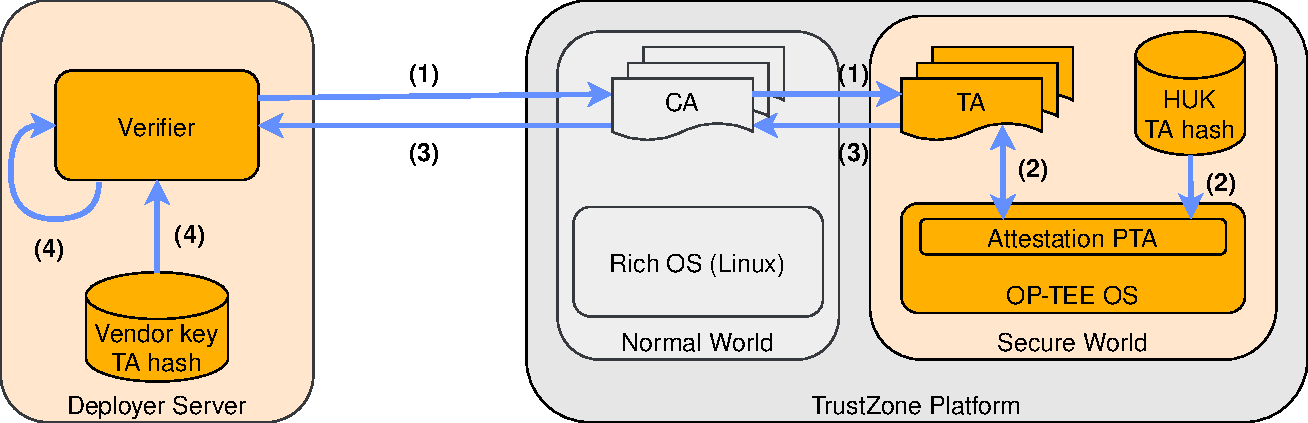
\includegraphics[width=\columnwidth]{graphics/trustzone-attestation.drawio.pdf}}}%
  {}%
  {Our remote attestation process for ARM TrustZone with OP-TEE. Colored
  components are considered trusted in our architecture.}%
  {fig:RA}

\subsubsection{Remote attestation and secure channels}
\label{impl:tz-attestation}

Remote attestation is a crucial security feature for our framework that provides
an authorized party with cryptographic proof that a known and benign TA is
initially loaded on a valid TrustZone device. In contrast to Sancus and Intel
SGX, the TrustZone specification offers no mechanism for remote attestation.
Some existing approaches leverage hardware components such as a hardware Trusted
Platform Module (\emph{TPM}) or a firmware-based TPM (e.g., Microsoft's
\emph{fTPM}~\cite{FTPM}) that provides security guarantees similar to a hardware
TPM, to perform attestation.  In our work we avoid the added complexity and
substantial increase of the TCB, and introducing no additional hardware. Instead
we propose an attestation mechanism based on native TrustZone features.

Our design is based on Sancus' remote attestation scheme (\cref{impl:sancus}).
Analogously, our approach relies on symmetric cryptography and a three-level key
hierarchy. We build upon an OP-TEE proof-of-concept implementation for remote
attestation that requires minimal hardware features and assumptions\footnote{See
\url{https://github.com/OP-TEE/optee\_os/issues/3189/} and
\url{https://github.com/OP-TEE/optee\_os/pull/4011/}. Very recently, attestation
is being picked up and included in release 3.17 (April 2022) by the OP-TEE team
again.}, avoiding the use of an TPM/fTPM as they are not available on many
platforms. We implemented an attestation protocol derived from the OP-TEE
proof-of-concept to address the requirements of our framework, while minimizing
the run-time TCB.

Our scheme assumes that each TrustZone device is equipped with a \ac{HUK} (also
called \emph{endorsement key} in other technologies), which can be created at
manufacture time and stored either in hardware fuses or the secure eMMC
partition. Similar to hardware devices like the TPM or Sancus, the \ac{HUK} is
protected from unauthorized access and can be used as root-of-trust of the
TrustZone device. Since the secure boot process guarantees system integrity,
OP-TEE can be treated as the trusted base for accessing the \ac{HUK}, and the
isolation properties provided by TrustZone protect secure-world code at
run-time. Thus, we get a strong guarantee that the \ac{HUK} can only be accessed
by privileged code in the secure world.

To leverage the \ac{HUK} and provide attestation primitives to the TAs, we
developed an attestation \ac{PTA}%
%
\footnote{\label{note:trustzone-ta}PTAs are an OP-TEE concept. They
	provide interfaces that are exposed by the OP-TEE Core to client TAs. See
	\url{https://optee.readthedocs.io/en/latest/architecture/trusted_applications.html}
	for more details.}
%
that is statically built into the OP-TEE core and runs at the same privileged
execution level as the OP-TEE OS. Analogous to Sancus attestation, this \ac{PTA}
uses a \ac{KDF} to retrieve symmetric vendor and module keys from the \ac{HUK}.
In particular, the vendor key is computed as follows:%
\[ vendor\_key := KDF(HUK \mathbin\Vert vendor\_id) \]
%
Identically to Sancus~(cf. Section~\ref{impl:sancus}), \texttt{vendor\_id} is a
unique identifier assigned to the software vendor, and the \texttt{vendor\_key}
needs to be securely communicated out-of-band. The \texttt{vendor\_id} is then
embedded in the TA code and passed to the \ac{PTA} during the attestation
process. The module key, instead, is computed as:%
\[ module\_key := KDF(vendor\_key \mathbin\Vert TA\_hash) \]
%
The TA hash is used by the OP-TEE OS to verify the integrity of the TA at load
time\footnote{The TA's binary structure and loading process are described in
detail at
\url{https://optee.readthedocs.io/en/latest/architecture/trusted_applications.html}.}.
We made minimal changes to the OP-TEE OS to store the hash in secure memory
after loading a TA, so that it could be retrieved by the attestation \ac{PTA}
for computing the module key. The module key can be also used to establish a
secure communication channel between the TA and the remote party.

Our remote attestation process shown in \cref{fig:RA} is illustrated in detail
as follows:
%
\begin{enumerate}
	\item The verifier sends an attestation request to the client application
	running in the normal world on the target device. The request contains a
	randomly generated \emph{challenge} to provide freshness. Then, the client
	application passes the received \emph{challenge} to the intended TA through
	shared memory.
	\item The TA leverages the attestation \ac{PTA} to obtain the module key
	\emph{K}. The attestation \ac{PTA} performs a double derivation to retrieve
	the module key from the \ac{HUK}, as explained above. To do so, the vendor
	identifier is passed as parameter by the TA itself, whereas the TA hash is
	fetched from secure memory. After receiving \emph{K}, the TA calculates a
	\ac{MAC} \emph{D} of the provided \emph{challenge}.
	\item The TA sends \emph{D} to the client application through shared memory
	and then \emph{D} is forwarded to the remote verifier. 
	\item The verifier derives the same module key \emph{K} from the vendor key
	and TA hash. Then, the verifier uses \emph{K} to compute a \ac{MAC} of
	\emph{challenge} and then compares it with the received \ac{MAC}. If the two
	values match, the target device is authenticated and the TA integrity is
	verified.
\end{enumerate}

The \ac{KDF} used in our proof-of-concept is a simple SHA-256 hash, though we
truncate the module key to 128 bits to align its size with the other \ac{TEE}
implementations. For \ac{MAC} function we leveraged the AES-128-GCM
authenticated encryption scheme, using the challenge as associated data.

Similarly to Sancus, attestation binds a TA to a specific node because the
module key is (indirectly) derived from the \ac{HUK}.
Deploying the TA on
a different node would result in a different module key. Since the TA's
UUID is hard-coded, multiple instances of the same TA would have different
hashes and consequently different module keys, provided that each instance uses
a different UUID.

This attestation scheme gives strong guarantees that a TA is running expected
code on a particular TrustZone node. The freshness of the challenge prevents
replay attacks, ensuring that the TA is up and running at the time of the
attestation. Adversaries cannot learn the module key by sniffing the network
traffic, nor can they impersonate a TA to compute the response to the challenge.
Besides, any attempt to modify the messages between TA and verifier would only
result in a failed attestation. However, the scheme relies on the security of
the \ac{HUK} and vendor key: if a \ac{HUK} is leaked, all TAs deployed on its
corresponding TrustZone node are compromised, while leaks of a vendor key
only compromises the TAs of its corresponding software vendor deployed on
its corresponding node. Hence, a device manufacturer should provide
software vendors with a secure interface (e.g., an authenticated API) to
retrieve the vendor key for a specific TrustZone node.

\subsubsection{Secure I/O}
%
TrustZone leverages dedicated hardware components to enforce hardware isolation
to the I/O devices.  Specifically, TrustZone introduces the TrustZone Protection
Controller to define the access restrictions for peripherals and configure them
as secure and non-secure dynamically or statically. This is achieved by the
reflection of Non-Secure bit into the respective peripheral. Several works take
the advantage of TrustZone to establish a trusted I/O path for different
purposes \cite{TrustUI, ProtectedConfirmation, TrustOTP, TrustPay}
(\cref{rel-work:secureio}). Our framework does not support physical I/O
channels for TrustZone-based modules yet but rather interfaces Sancus-enabled
I/O devices.

\newcommand{\pie}[1]{%
\begin{tikzpicture}
 \draw (0,0) circle (1ex);\fill (1ex,0) arc (0:#1:1ex) -- (0,0) -- cycle;
\end{tikzpicture}%
}

\newcommand{\revpie}{%

\begin{tikzpicture}
 \draw (0,0) circle (1ex);\fill (0,1ex) arc (90:270:1ex) -- (0,0) -- cycle;
\end{tikzpicture}%
}

\newcommand{\rot}[1]{\rotatebox{#1}}
\newcommand{\CIRCLE}{\pie{360}}
\newcommand{\Circle}{\pie{0}}
\newcommand{\LEFTcircle}{\pie{180}}
\newcommand{\RIGHTcircle}{\revpie}


\begin{table}
    \newcommand{\rh}[1]{\rot{33}{\textbf{#1}}}
    \newcommand{\yes}{\CIRCLE}
    \newcommand{\pa}{\LEFTcircle}
    \newcommand{\no}{\Circle}
    \newcommand{\na}{\makebox[8pt][c]{\textbf{--}}}
    \newcommand{\po}{{\LEFTcircle}}
    \newcommand{\tzfootnote}{\textsuperscript{a}}
    \newcommand{\tzfootnotetext}{We consider TrustZone with the OP-TEE OS and our extensions for attestation}

    \newcolumntype{a}{p{5mm}}
    \setlength{\tabcolsep}{1mm}

     \label{tbl:tee-comparison}
      \resizebox{0.7\textwidth}{!}{
	    \begin{tabular}{@{}l@{\hskip 5mm}aaaaaaa@{\hskip 15mm}aaaa@{\hskip 15mm}r@{}}
	        & \rh{Isolation} & \rh{SW Attestation} & \rh{TCB Attestation} & \rh{Memory Protection} &  \rh{Sealing} & \rh{Code Confidentiality} & \rh{Secure I/O} & \rh{HW-Only TCB} & \rh{Upgradeable TCB} & \rh{Preemption} & \rh{Dynamic Layout}  & \textbf{Target ISA} \\ \midrule
            \textbf{Sancus}                 & \yes & \yes & \yes  & \no  & \no  & \po  & \yes & \yes & \no  & \po  & \no  & MSP430 (16-bit) \\ \midrule
            \textbf{SGX}                    & \yes & \yes & \yes  & \yes & \po  & \po  & \po  & \no  & \yes & \yes & \yes & x86\_64 (64-bit) \\ \midrule
            \textbf{TrustZone\tzfootnote}   & \yes & \yes & \yes  & \no  & \po  & \po  & \po  & \no  & \yes & \yes & \yes & ARM (32-bit) \\
	        \bottomrule \\
    	    \multicolumn{13}{c}{\yes\xspace= Yes; \po\xspace= Possible; \no\xspace= No} \\
	    \end{tabular}
	}

    \caption{Comparison of \ac{TEE} hardware features and the resulting security
    guarantees and application capabilities in our framework. This table is
    derived and adapted from~\cite{maene:hardware}.
    \emph{Footnotes --- } 
    \tzfootnote{}: \tzfootnotetext.
    \vspace{-1em}
   }
\end{table}



\subsection{Comparison: \acp{SM} on different \acp{TEE}}
\label{impl:comparison}

\cref{tbl:tee-comparison} summarizes the features of each \ac{TEE} and
highlights their main differences. This table is derived and adapted from
\cite{maene:hardware}. Note that for TrustZone we consider OP-TEE OS with our
attestation extensions.
The key points that distinguish our \acp{TEE} are \emph{a)} software isolation
which is supported by all three \acp{TEE} and where we provide common
interfaces to control isolation and event handling;
\emph{b)} attestation primitives, which are not available on all \acp{TEE} and we 
provide attestation support as necessary and establish common Attest entry
point and event handler abstracting for our framework; and \emph{c)}
secure I/O, which is only natively supported with Sancus and where we
design generic scheme that can hopefully be instantiated by other
\acp{TEE}, in particular by ARM TrustZone.

Software isolation and attestation are strict requirements in our design
(\cref{design:tee}), which are fully satisfied by Intel \ac{SGX} and Sancus. For
TrustZone, instead, we relied on OP-TEE OS for isolation, whereas we designed
and implemented our own attestation protocol based on Sancus
(\cref{impl:tz-attestation}). Other than code integrity and authenticity,
attestation may also provide additional information, such as the security
configuration of the underlying TCB (Intel \ac{SGX}), or the guarantee that an
\ac{SM} is running on a specific node (Sancus and TrustZone). The latter is
particularly useful when dealing with driver modules
(\cref{concept:protected-drivers}). Besides, only Intel \ac{SGX} protects the
integrity and authenticity of data from physical attacks, thanks to its Memory
Encryption Engine (MEE).

Both Intel \ac{SGX} and TrustZone support sealing, i.e., storing data securely
on permanent storage. However, our framework does not currently provide any
abstraction over sealing primitives, meaning that developers need to manually
implement code to call such primitives. Similarly, code confidentiality (i.e.,
deploying encrypted \acp{SM} in order to protect sensitive code and static data)
is a feature supported by all architectures, though not essential for the use
cases we consider. Nevertheless, both sealing and code confidentiality could be
addressed in future work. Besides, Sancus fully supports secure I/O
(\cref{concept:secure-io-sancus}), while on TrustZone and Intel \ac{SGX} some
extensions are needed, as proposed in related work (\cref{rel-work:secureio}).

Concerning architectural features, only Sancus provides an hardware-only trusted
computing base. In fact, Intel \ac{SGX} relies on software parts such as
microcode and attestation enclaves, while TrustZone includes the whole OP-TEE
operating system in its \ac{TCB}. However, software can be easily upgraded to
provide new functionalities or fix bugs, which is why Intel \ac{SGX} and
TrustZone support \ac{TCB} upgrades. Furthermore, both TrustZone and Intel
\ac{SGX} have full support for interrupts and dynamic layout (i.e., virtual
memory). Sancus, being an embedded \ac{TEE}, does not support virtual memory,
whereas for interrupts we offer partial support
(\cref{concept:secure-io-sancus}).

\subsection{Deployment}
%
\label{impl:deployment}

We developed a Python script called \reactools{} to ease the deployment and
initialization of a distributed application. In essence, this script
builds the \protmods{} and then communicates with the remote event managers to
bootstrap enclaves and establish connections (\cref{concept:untrusted-sw}).
\reactools{} takes as input a \emph{deployment descriptor}, a configuration file
that contains a high-level description of the application to deploy. 

\subsubsection{Deployment descriptor} 

\sclist{0.5}%
  {\lstinputlisting[language=Yaml]{descriptor.yaml}}%
  {}%
  {Excerpt from a deployment descriptor in YAML format. Three main sections are
  defined: \code{nodes}, \code{modules} and \code{connections}. Each node and
  module has a \code{type} field indicating the \ac{TEE} technology used;
  besides the fields that are common to all \acp{TEE}, each platform also
  requires other specific parameters. The fields of a connection, instead, do
  not change. The complete deployment descriptor (in JSON format) used in this
  example  can be found at
  \url{https://github.com/AuthenticExecution/examples/blob/main/button-led/descriptor.json}.}%
  {code:descriptor}

The deployment descriptor contains three main sections: \code{nodes},
\code{modules} and \code{connections}. \cref{code:descriptor} shows an excerpt
from one of our sample applications. 

As shown in the figure, a module is statically assigned to a node and a specific
\ac{TEE} technology. This is a limitation of our framework as each \ac{TEE}
implementation uses its own API and programming language. A possible direction
for future work could be to use an unified language for defining modules, which
can be an existing programming language such as Rust or a custom language such
as the pseudocode we used in \cref{code:examples}; then, the framework could
automatically select the right compiler/toolchain according to the node in which
the \ac{SM} is going to be deployed. However, it is worth noting that not all
\acp{TEE} provide the same features: for example, Intel \ac{SGX} supports data
sealing, whereas Sancus does not support persistent storage at all.

In the \code{connections} section, the deployer declares connections between
\protmods. A connection links together two endpoints, each of them identified by
the pair \emph{<SM\_name,endpoint\_name>}. Moreover, each connection must
indicate the authenticated encryption algorithm to use for protecting events in
transit. Currently, both Intel \ac{SGX} and TrustZone support \aes-\ac{GCM} and
\spongent{} (both with 128 bits of security), whereas Sancus only supports
\spongent{}.

\subsubsection{Deploying a new application}

\reactools{} provides separate commands for the deployment and attestation of
modules, as well as for the establishment of connections. To this end, the
deployer would run the \cmd{deploy}, \cmd{attest}, and \cmd{connect} commands in
sequence, each time providing as input the same deployment descriptor. If all
these commands succeed, the deployment is complete and the application is ready
to process events.

\subsubsection{Interfacing with the application}
%
\label{impl-descriptor-interfacing}

At runtime, the deployer might want to interact with the application in a secure
way, e.g., to initialize a web server or to get some metrics from a database.
However, the \callentry{} API provided by the event managers to call modules'
entry points is not secure, as for this kind of message the data is transmitted
unencrypted over the network. Hence, the deployer would need to manually
implement encryption and/or authentication mechanisms for data exchanged with
the application.

Nevertheless, to facilitate the secure communication between a deployer and
their \protmods, our framework provides a convenient feature called \emph{direct
connections}. Unlike normal connections between two modules, a direct connection
uses the deployer's machine as source endpoint. Since connection keys are
generated and distributed at deployment time by our script, it is possible to
also use such keys to generate output (or request) events and send them directly
to running modules.

These connections can be defined in the deployment descriptor together with the
others, and are characterized by the additional \code{direct:true} field. The
deployer can then either generate new events manually or automatically using
\reactools; either way, the receiving module processes these events just as any
other event. Since the deployer's machine is assumed to be trusted, the same
security guarantees as normal connections apply for direct connections as well.

\subsection{Attestation and key management}
\label{impl:attestation}

To ease the attestation of modules and the storage of encryption keys, we
developed an optional component called the \emph{Attestation Manager}. It
consists of an Intel \ac{SGX} enclave that is deployed on the infrastructure
together with the applications, and to which the deployer and \reactools{} can
send requests through a dedicated command-line interface.

When the attestation manager is deployed, it first needs to be attested using
the usual Intel \ac{SGX} attestation process. Similarly to the attestation of
\protmods, a shared secret is exchanged between the challenger (i.e., the
deployer) and the enclave, which is then used to establish a secure channel.

After the initialization is complete, the attestation manager is ready to
receive \attest{} requests from the deployer; the attestation manager then takes
care of executing the actual attestation logic, based on the \ac{TEE} technology
used by the module. If the attestation succeeds, the attestation manager stores
the module key securely in the enclave memory, and it can be fetched (or used
indirectly) by the deployer at any time.

\subsubsection{Advanced usages} 
%
The attestation manager, when used, may enable additional use cases. Below, we
shortly describe some of them. Note that we only aim to provide an informal and
high-level outline of such use cases, to motivate the usage of a centralized
attestation/key management component. As such, we will not go into details on
the design nor perform a security analysis.

\begin{itemize}
  \item \textit{Key management.} The simplest use case is to merely store
  credentials (i.e., module and connection keys), which can be accessed by the
  deployer or any other authorized entities when needed. Credentials can be
  stored in enclave memory or persisted in storage using sealing capabilities of
  \acp{TEE} such as Intel \ac{SGX}. Note that the latter case may introduce
  vulnerabilities against rollback attacks \cite{alder2018migrating}.
  %
  \item \textit{Distributed confidential computing.} Certain applications
  process privacy-sensitive information, such as health-related
  data. \acp{TEE} already protect against honest-but-curious infrastructure
  providers, while attestation ensures the authenticity of application code and
  proves that the isolation mechanisms of a \ac{TEE} are correctly in place.
  However, in some cases it may be desirable to conceal sensitive data even from
  the deployer, who normally has access to connection keys and could potentially
  decrypt data in transit between modules. Therefore, the attestation manager
  could be used to generate and distribute connection keys to modules without
  the deployer learning any information about their value.
  %
  \item \textit{Root of Trust in edge devices.} In some edge scenarios such as
  automotive/\ac{V2X}, nodes may be part of a local network
  that does not have continuous access to Internet services. In such cases, it
  might be useful to deploy an attestation manager on the network responsible
  for the initialization and attestation of local enclaves. For instance, we
  could envision a TrustZone gateway in a car that initializes all Sancus'
  \acp{ECU} when the engine is turned on, refusing to start the car if any of
  the attestations fails \cite{vanbulck_2017vulcan}. In this scenario, the
  gateway acts as the \textit{root of trust} of the system, and its remote
  attestation would be possible as soon as the system comes back online.
\end{itemize}
